\documentclass{article}
\usepackage[final]{neurips}
\usepackage[framemethod=tikz]{mdframed}
\usepackage{lipsum,amsthm,amssymb}
\definecolor{mycolor}{rgb}{0.122, 0.435, 0.698}
\newmdenv[innerlinewidth=0.5pt, roundcorner=4pt,linecolor=mycolor,innerleftmargin=6pt,
innerrightmargin=6pt,innertopmargin=6pt,innerbottommargin=6pt]{mybox}
\usepackage[utf8]{inputenc} % allow utf-8 input
\usepackage[T1]{fontenc}    % use 8-bit T1 fonts
\usepackage{hyperref}       % hyperlinks
\usepackage{url}            % simple URL typesetting
\usepackage{booktabs}       % professional-quality tables
\usepackage{amsfonts}       % blackboard math symbols
\usepackage{nicefrac,tcolorbox}       % compact symbols for 1/2, etc.
\usepackage{amsmath}
\usepackage{enumitem}
\usepackage{microtype}      % microtypography
\usepackage{graphicx,caption}
\usepackage{xepersian}
\settextfont{XB Niloofar}
\setdigitfont{XB Niloofar}
\raggedbottom


\title{
	\vspace{-0.8em}
تمرین سری چهارم درس نظریه گروه‌ها - دکتر رضاخانی
\\
{\normalsize
\textbf{مهلت تحویل:
شنبه ۲۵ فروردین ماه سال 1403 تا ساعت 59:23
\\
\vspace{-0.4em}
از طریق سامانه
\href{https://cw.sharif.edu/}{درس‌افزار شریف}
}
}
\vspace{-0.6em}
}

\usepackage[utf8]{inputenc}

\usepackage[english]{babel}
\setlength{\parindent}{3.5em}
\setlength{\parskip}{0.5em}
\renewcommand{\baselinestretch}{1.0}

\usepackage{calrsfs}
\DeclareMathAlphabet{\pazocal}{OMS}{zplm}{m}{n}
\newcommand{\La}{\mathcal{L}}
\newcommand{\Lb}{\pazocal{L}}

\newtcolorbox{boxes}[3][]
{
	colframe = #2!25,
	colback  = #2!10,
	coltitle = #2!40!black,  
	title    = {\textbf{#3}},
	#1,
}

\newenvironment{exercise}[3][\unskip]{%
	\par
	\noindent
	\textbf{تمرین
		#1
		[#2 امتیاز] 
		\def\temp{#3}\ifx\temp\empty
		: 
		\else
		: #3 \vspace{0.5em} \\ \noindent
		\fi
}}{}


\author{
حسین محمدی\\
  \lr{
  		\href{mailto:hossein.mohammadi.00427@gmail.com}{\texttt{	hossein.mohammadi.00427@gmail.com}}} \\
  \And
  زهرا کبیری\\
 \lr{
  		\href{mailto:kabiri.zahra98@gmail.com}{ \texttt{kabiri.zahra98@gmail.com}}}\\
  }

\begin{document}


\begin{minipage}{0.1\textwidth}% adapt widths of minipages to your needs
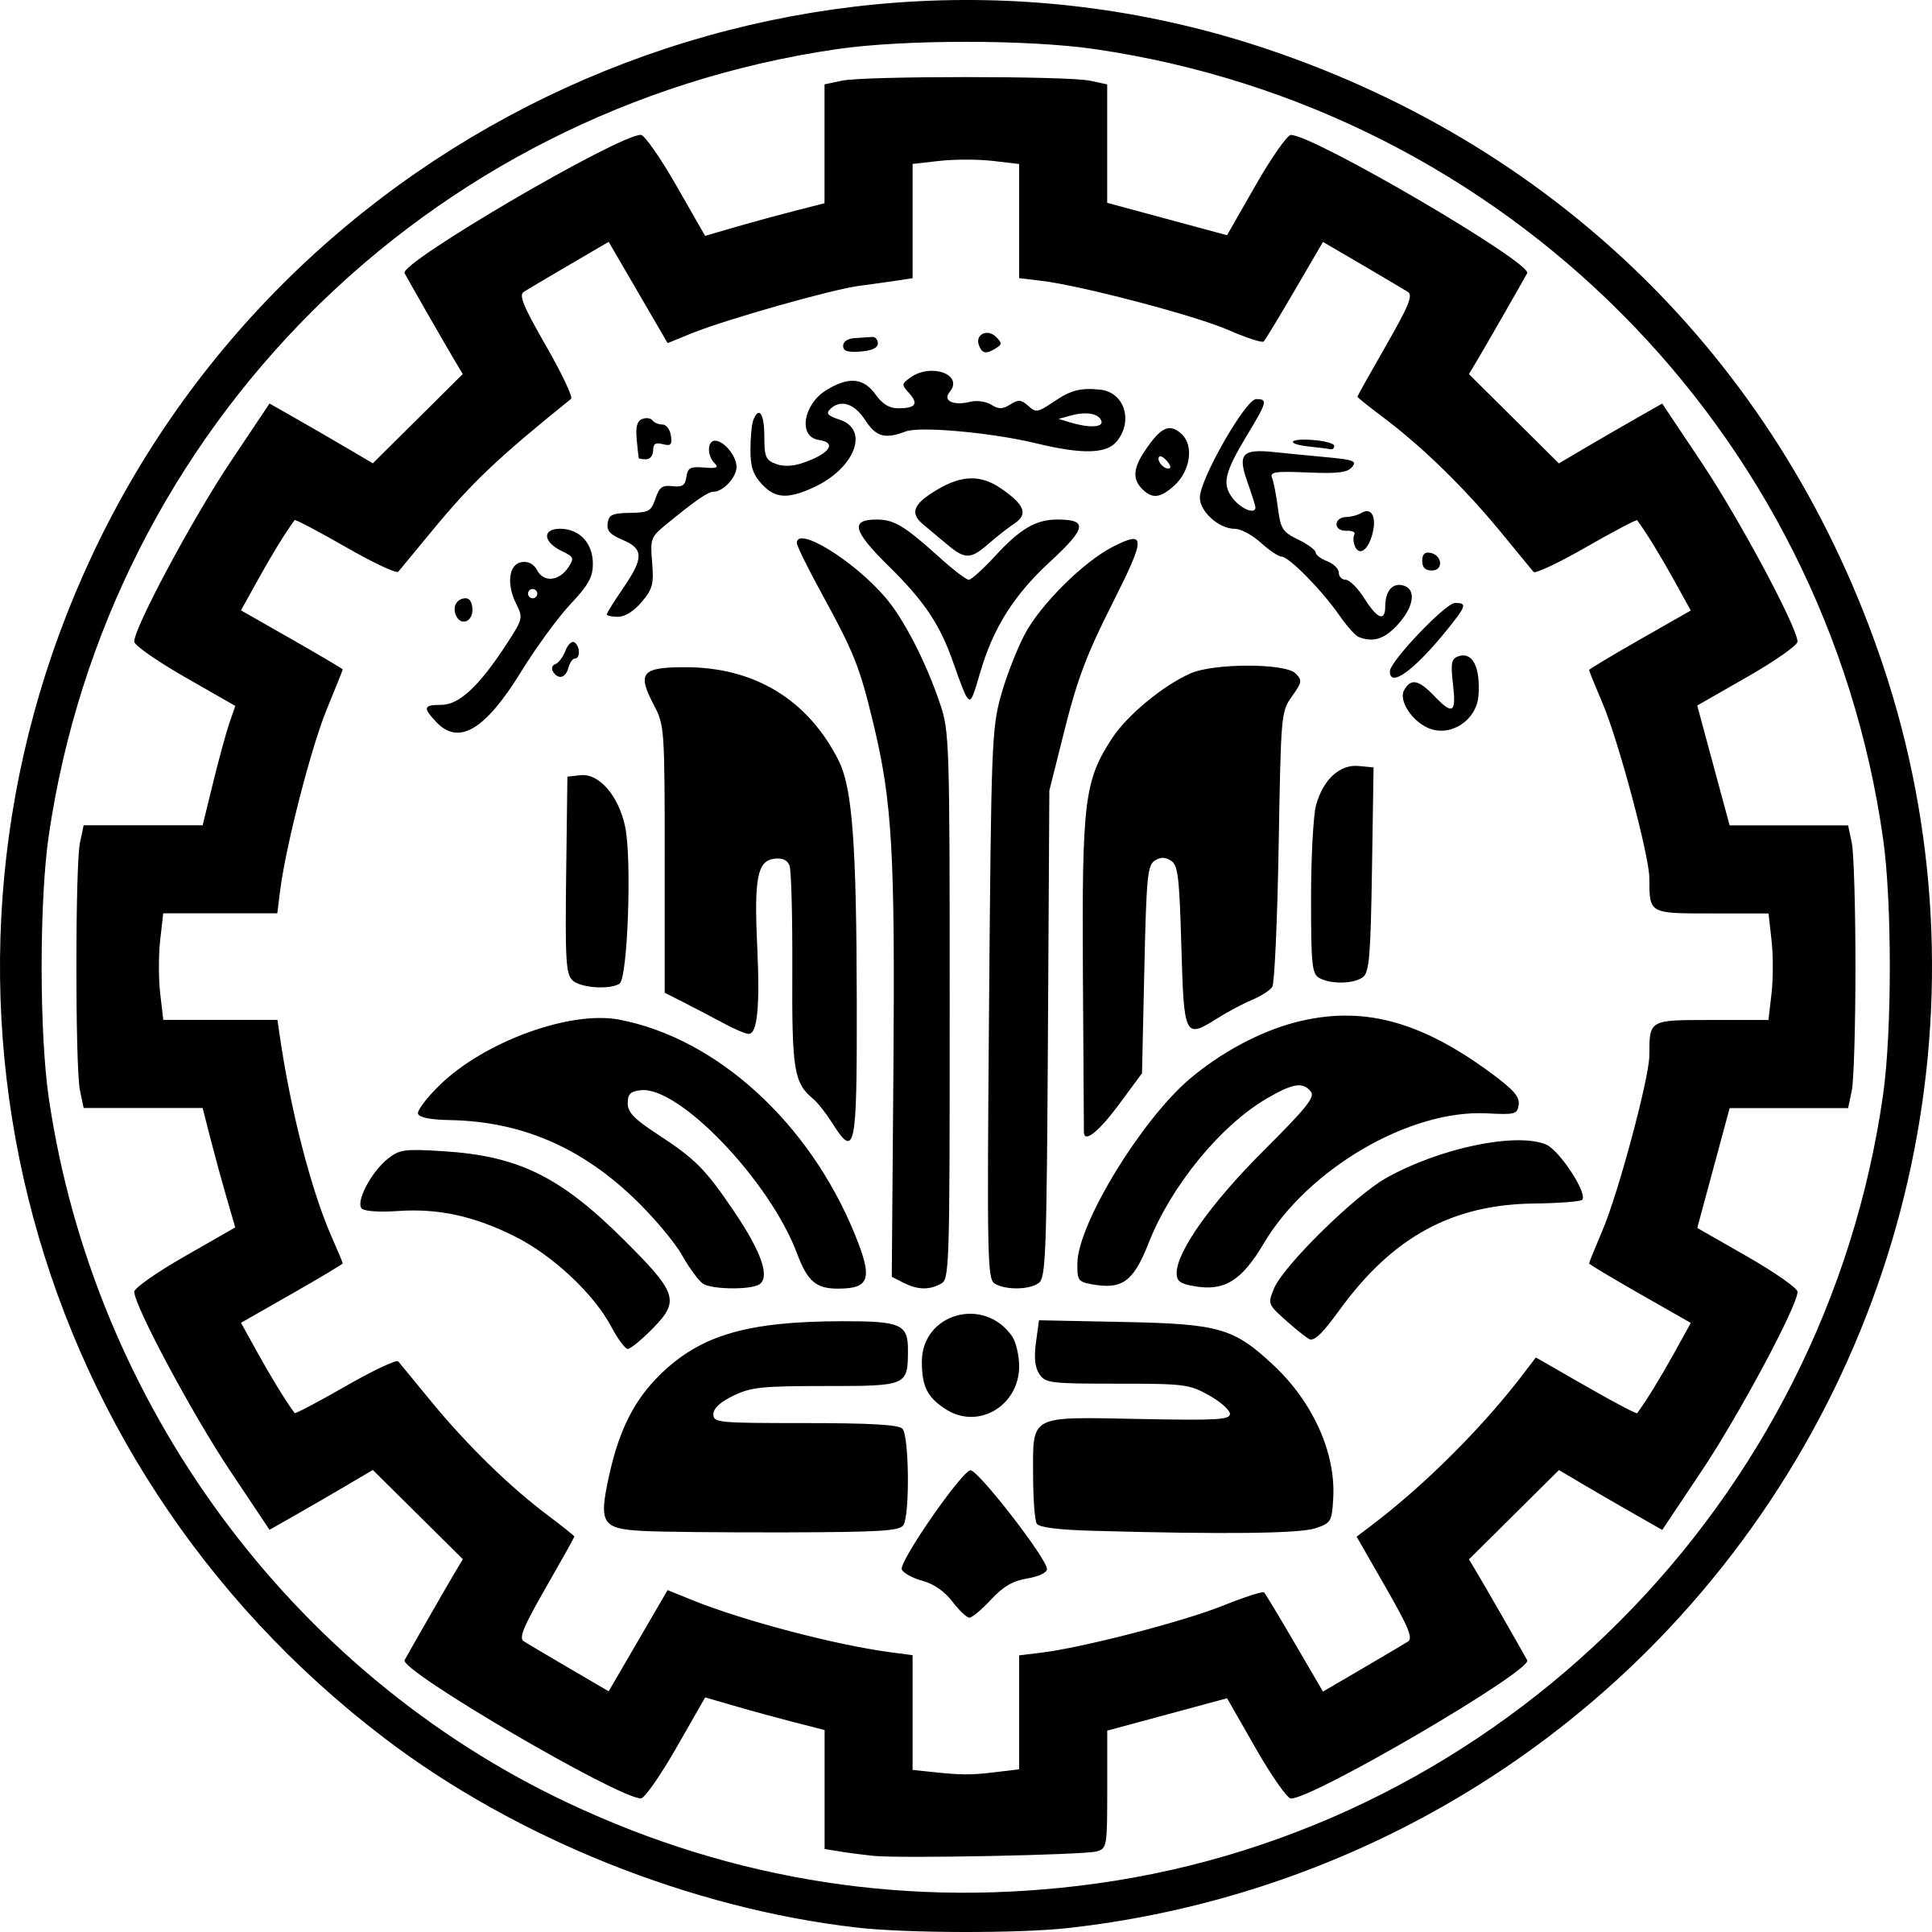
\includegraphics[width=1.1cm]{sharif-logo.png}
\end{minipage}%
\hfill%
\begin{minipage}{0.9\textwidth}\raggedleft
دانشگاه صنعتی شریف\\
زمستان ۱۴۰۲ - بهار ۱۴۰۳\\
\end{minipage}

\makepertitle


\begin{exercise}[15]{20}{قضیه اساسی همریختی}
حالا که با زیرگروه بهنجار آشنا شدید؛ می‌توانیم قضیه‌ای اساسی و مهم را بیان و اثبات کنیم.	

\noindent
\textbf{قضیه اول همریختی:}
دو گروه 
$(G_1,\times_1)$
و
$(G_2,\times_2)$
با همریختی
$\varphi: G_1 \longmapsto G_2$
 بین آنها مفروض‌اند. آن‌گاه
\[
\frac{G}{\ker \varphi} \simeq \text{im} \; \varphi
\]
	که $\ker \varphi$ و $ \text{im} \; \varphi$ به‌ترتیب هسته و تصویر همریختی 
	$\varphi$
	هستند.
	
	\noindent
	الف) اول نشان دهید که هسته‌ی همریختی یک زیرگروه بهنجار از 
	$G$
	است؛ یعنی 
	$\ker \varphi \trianglelefteq G$.
	
	\noindent
	ب) نگاشت 
	$\Phi:\frac{G}{\ker \varphi} \longmapsto \text{im} \; \varphi$
	 که اعضای گروه خارج قسمتی را به تصویر نگاشت 
	$\varphi$
	می‌نگارد، اینطور معرفی می‌کنیم:
	\[
	\Phi (g \ker\varphi) := \varphi(g).
	\]
خوش تعریفی این نگاشت را نشان دهید؛ یعنی اگر 
$g\ker\varphi = g'\ker\varphi$
یک عضو از گروه خارج‌قسمتی باشد که با نماینده‌های متفاوتی نشان داده شده‌است، تحت نگاشت 
$\Phi$
به یک عضو از تصویر نگاشته می‌شوند.

\noindent
ج) ثابت کنید که 
$\Phi$
 همریختی گروهی است. همچنین نشان دهید که این نگاشت یک‌به‌یک و پوشاست.


\noindent
بنابراین $\Phi$ یکریختی است و نتیجه می‌شود که گروه مبدا و مقصد با هم یکریخت هستند.
\end{exercise}



\begin{exercise}[۱۶]{15}{زیرگروه‌های بهنجار تو‌درتو
	\LTRfootnote{Nested normal subgroups}
	}
با ذکر یک مثال نشان دهید که می‌توانیم  زیرگروه‌های تودرتوی $E\leq F \leq G $  را به گونه‌ای پیدا کنیم که 
$E \trianglelefteq F$
و
 $F \trianglelefteq G$
 اما  
 $E \ntrianglelefteq G$
 \footnote{مقصود از نمادگذاری
 $G_1 \trianglelefteq G_2$
 این است که زیرگروه $G_1$ در گروه $G_2$ بهنجار است. همچنین
  $G_1 \ntrianglelefteq G_2$
  یعنی زیرگروه $G_1$ در گروه $G_2$ بهنجار نیست.
 }.
\end{exercise}


\begin{exercise}[۱۷]{15}{}
گروه 
$G$ 
را که از ماتریس‌های 
$2\times 2$ 
به صورت 
$\biggl\{\begin{pmatrix}
		a & b \\
		0 & d 
\end{pmatrix}
\;\Big|\; a,b,c \in \mathbb{R}\; ,\; ad \neq 0
\biggr\}
$
تشکیل شده با ضرب ماتریسی در نظر بگیرید.
مجموعه‌ی 
$N=\biggl\{\begin{pmatrix}
		1 & b \\
		0 & 1 
\end{pmatrix}\;\Big| \; b\in \mathbb{R}\biggr\}$ 
را نیز در نظر بگیرید. 
نشان دهید: 

\noindent
الف) 
$N$ 
یک زیرگروه بهنجار 
$G$ 
است. 

\noindent
ب) گروه خارج قسمتی
$G/N$ 
جابه‌جایی
\LTRfootnote{Abelian} 
است.
\end{exercise}


\begin{exercise}[۱۸]{25}{}
فرض کنید 
$H$ 
و 
$K$ 
دو زیرگروه بهنجار از گروه 
$G$ 
باشند به طوری که 
$H \cap K = \{e\}$. 

\noindent
الف)‌ نشان دهید برای هر 
$h \in H$ 
و هر 
$k \in K$ 
داریم 
$hk=kh$.

\noindent
ب)اول مطابق مطالبی که در کلاس حل تمرین دیدید؛ استدلال کنید که 
$HK$
یک زیرگروه از $G$ است؛ سپس  
 نشان دهید حاصل ضرب دکارتی 
$H \times K$ 
با گروه 
$HK$ 
یکریخت است. 
\begin{equation*}
HK=\{hk | \forall h \in H \; , \; \forall k \in K \}
\end{equation*}

\end{exercise}

\vspace{1em}

\begin{boxes}{black}{تعریف شاخص یک زیرگروه}
	شاخص
		\LTRfootnote{Index of a subgroup}
	 یک زیرگروه $H\leq G$
	را با 
	$[G:H]$
	نشان می‌دهیم و مقدارش تعداد هم‌مجموعه‌های 
	$H$ در $G$ است
	.
	\[
	[G:H] = \frac{|G|}{|H|}
	\]
  در تعریف بالا، تفاوتی نمی‌کند که منظورمان از هم‌مجموعه، هم‌مجموعه‌‌ی راست باشد یا هم‌مجموعه‌ی چپ
 \footnote{توجه کنید که تعداد هم‌مجموعه‌های راست و چپ با هم برابرند؛ این لزوما به این معنی نیست که هر هم‌مجموعه‌ی راست با یک هم‌مجموعه‌ی چپ برابر است.}.
	
	\vspace{0.6em}
	\textbf{استدلال:}
	اگر تعداد هم‌مجموعه‌های راست و چپ را به ترتیب با
	$[G:H]_r$
	و
	$[G:H]_l$
	نشان بدهیم؛ باید ثابت کنیم که این‌دو باهم برابرند.
	نگاشت زیر را در نظر بگیرید:
	\[
	f(X) = X^{-1}
	\]
	این نگاشت روی هم‌مجموعه‌های چپ اثر می‌کند و آن‌ها را به هم‌مجموعه‌ی راست می‌نگارد.
	
	می‌توانیم ببینیم که 
	\[
	f(g_iH)=Hg_i^{-1}
	\]
	از این مشاهده، به سادگی نتیجه می‌شود که این نگاشت، یک‌به یک و پوشاست (به عنوان تمرینی ساده دست به قلم شوید.)؛
	بنابراین، تعداد هم‌مجموعه‌های چپ و راست با هم برابرند.
	\qed
	
	یک رابطه‌ی جالب دیگر برای شاخص گروه‌ها وجود دارد که تحت عنوان «رابطه برج
	\LTRfootnote{Tower Law}
	» شناخته می‌شود.

\vspace{0.6em}
\textbf{قضیه برج
	\footnote{برای اثبات به 
	\href{https://proofwiki.org/wiki/Tower_Law_for_Subgroups}{این صفحه}
	رجوع کنید.}
	:}
اگر 
$K\leq H\leq G$
زیرگروه‌هایی با اندیس متناهی باشند؛ آن‌گاه
$[G:K] = [G:H][H:K]$.
\end{boxes}
\vspace{1em}

\begin{exercise}[۱۹]{10}{شرط‌‌های بهنجاری یک زیرگروه}
	الف) فرض کنید 
	$H$ 
	تنها زیرگروه با مرتبه 
	$\mathcal{O}(H)$ 
	از گروه متناهی 
	$G$ 
	است. نشان دهید که 
	$H$ 
	یک زیرگروه بهنجار از
	$G$ 
	است. 
	
	\noindent
	ب)
	اگر 
	$G$ 
	یک گروه باشد و 
	$H$ 
	یک زیرگروه با شاخص ۲ در 
	$G$ 
	باشد. نشان دهید که 
	$H$ 
	یک زیرگروه بهنجار 
	$G$ 
	است.
	
	\noindent
	(
	\textbf{راهنمایی:}
	از تعاریف دیگر زیرگروه بهنجار استفاده کنید؛ تعریفی از زیرگروه بهنجار هست که حل این سوال را بسیار ساده می‌کند.
	)
\end{exercise}

\begin{exercise}[20]{15}{}
	دو زیر گروه 
	$H_1$ 
	و 
	$H_2$ 
	از گروه 
	$G$ 
	را در نظر بگیرید. نشان دهید هر هم‌مجموعه راست نسبت به 
	$H_1 \cap H_2$ 
	خود اشتراک یک هم‌مجموعه راست 
	$H_1$ 
	با هم‌مجموعه راست دیگری از 
	$H_2$ 
	است. از این نتیجه استفاده کنید تا قضیه پوانکاره را اثبات کنید. 
	\begin{mdframed}
		قضیه پوانکاره:‌ اگر 
		زیرگروه‌های 
		$H_1$ 
		و 
		$H_2$ 
		شاخص متناهی در 
		$G$ 
		داشته باشند، آن‌گاه اشتراک آن‌ها 
		($H_1 \cap H_2$) 
		نیز شاخص متناهی دارد.
	\end{mdframed}
\end{exercise}



\newpage
\begin{boxes}{black}{گروه جایگشت‌ها را بهتر بشناسیم.}
	در این جعبه، با خواص گروه جایگشت و اعضایش بیشتر آشنا می‌شویم.
	\subsection*{ماتریس‌های جایگشت}
	می‌توانیم جایگشت‌ها را با ماتریس ها هم نمایش دهیم. برای هر عضو $\sigma \in S_n$، مطابق دستور زیر، ماتریس متناظر با این عضو، 
	$(M_\sigma)_{\tiny n\times n}$، را پیدا می‌کنیم.
	\[
	\big(M_\sigma\big)_{ij} = \begin{cases}
		1 & \quad\quad \sigma(j) = i \\
		0 &\quad\quad {otherwise}.
	\end{cases}
	\]
	به عنوان مثال، ماتریس منتاظر با عضو
	\[
	\sigma =
	\begin{pmatrix}
		1 & 2 & 3 & 4 & 5 \\
		3 & 1 & 2 & 5 & 4 
	\end{pmatrix}
	\]
	به شکل زیر است:
	\[
	M_\sigma = \begin{pmatrix}
		0 & 1 & 0&0&0 \\
		0 & 0 &1&0&0 \\
		1&0&0&0&0 \\
		0&0&0&0&1\\
		0&0&0&1&0
	\end{pmatrix}
	\]
	می‌توانید با تعریف بالا مشاهده کنید که ترکیب جایگشت ها معادل با ضرب ماتریسی است. پس می‌توانید یک یکریختی بین گروه جایگشت و یک گروه از ماتریس‌های
	$n\times n$
	با درایه‌های 
	$\{0,1\}$
	تعریف کنیم.
	
	\textbf{نکته:}
	ماتریس 	$M_\sigma$ در هر سطر یا در هر ستونش، دقیقا یک درایه ۱ دارد.  با جابه‌جا کردن سطرهای ماتریس 
	$M_\sigma$
	می‌توانیم به ماتریس همانی برسیم، بنابراین دترمینان این ماتریس $\pm 1$ است. به طور خاص، در مورد ترانهش‌ها، که تنها جای دوسطر با هم عوض شده‌اند؛ دترمینانِ ماتریسِ متناظر با یک ترانهش، همواره منفی یک است.
	
	
	\subsection*{تعریف نگاشت
	\text{sgn}
	}
	حتما تا به حال اسم جایگشت‌های زوج یا فرد به گوش‌تان خورده است. در این بخش سعی می‌کنیم این اصطلاحات را دقیق‌تر بشناسیم.
	اول به قضیه زیر توجه کنید.
	
	\vspace{0.6em}
	\textbf{قضیه:}
	\textit{اگر 
	$\sigma\in S_n$
	دارای دو تجزیه‌ی 
	\[
	\begin{aligned}
		\sigma &= \alpha_1 \dots \alpha_r \\
		\sigma &= \beta_1 \dots \beta_s
	\end{aligned}
	\]
	به حاصل‌ضرب ترانهش‌ها باشد؛ آنگاه 
	$r \stackrel{2}{\equiv} s$.
	}
	
	\vspace{0.6em}
	\textbf{اثبات:}
	مطابق بخش قبلی، کافی ‌است که فقط ماتریس‌های متناظر با این دو تجزیه را تشکیل دهیم:
	\begin{equation*}
		\begin{aligned}
			A_\sigma =& A_{\alpha_1} \dots A_{\alpha_r} \\
			A_\sigma =& A_{\beta_1} \dots A_{\beta_s} 
		\end{aligned}
	\end{equation*}
	پس دترمینان این نمایش‌های ماتریسی بدست می‌آید:
	\begin{equation*}
		\begin{aligned}
		\det	A_\sigma =& \det(A_{\alpha_1}) \dots \det(A_{\alpha_r}) \\
		\det	A_\sigma =& \det(A_{\beta_1}) \dots \det(A_{\beta_s} )
		\end{aligned}
	\end{equation*}
	حالا، چون $\alpha_i$ و $\beta_j$ ها ترانهش هستند؛ پس دترمینان نمایش ماتریسی‌شان منفی یک است، بنابراین:
	\begin{equation*}
		\begin{aligned}
			\det (A_\sigma) &= (-1)^r \\
			\det (A_\sigma) &= (-1)^s
		\end{aligned}
	\end{equation*}
	پس شرط 
	$(-1)^r = (-1)^s$
	حاصل می‌شود که نتیجه‌ی $r \stackrel{2}{\equiv} s$
	را به دست می‌دهد. 
	\qed
\end{boxes}

\begin{boxes}{black}{گروه جایگشت‌ها را بهتر بشناسیم.}
	
	علامت یک جایگشت را به شکل زیر تعریف می‌کنیم:
	\begin{equation*}
		\text{sgn} (\sigma) = \begin{cases}
			1 & \quad \quad   \text{حاصل‌ضرب تعداد زوجی ترانهش باشد.}\; \sigma \\ 
			-1 & \quad \quad   \text{حاصل‌ضرب تعداد فردی ترانهش باشد.}\; \sigma
		\end{cases} 
	\end{equation*}
	
	قضیه‌ی فوق، خوش تعریفی نگاشت \lr{sgn} را نتیجه می‌دهد؛ اگر تجزیه یک جایگشت به ترانهش‌ها پاریته یکسان نداشته باشد، تحت این نگاشت باید به $\pm 1$ برود.
	
	حال بحث می‌دهیم که تعریف بالا، یک به‌روریختی
	\footnote{یعنی یک همریختی که پوشاست.}
	از گروه جایگشت‌ها به گروه
	$\{1,-1\}$
	با عمل ضرب (یعنی همان گروه دوری از مرتبه ۲) است.
	دلیل آن ساده است؛ اگر دو عضو زوج از گروه جایگشت‌ برداریم، تحت نگاشت 
	\lr{sgn}
	هر دو به یک نگاشته‌ می‌شوند. پس حاصل‌ضربشان این دو عضو (که به شکل تعداد زوجی ترانهش نوشته می‌شود) به عضو $1\times 1$ نگاشته می‌شود. بقیه موارد هم به طور مشابه استدلال می‌شوند. همچنین این نگاشت پوشاست چون این نگاشت یک ترانهش را به عضو $-1$ می‌نگارد.
	
	\vspace{0.8em}
	حالا بیایید قضیه اساسی همریختی که در بالا ذکر شد را به کار ببریم. می‌دانیم که هسته‌ی این نگاشت، اعضایی هستند که به ۱ نگاشته می‌شوند، یعنی تمامی جایگشت‌های زوج هسته‌ی این نگاشت هستند.
	\[
	\ker \text{sgn} := A_n = \{\sigma \in S_n \big| \text{sgn}(\sigma) = 1\}
	\]
	پس مطابق قضیه اول همریختی:
	\[
	\frac{S_n}{A_n} \simeq \mathbb{Z}_2
	\]
	این رابطه نتیجه می‌دهد که 
	$|A_n| ={ \frac{|S_n|}{2}}$
	؛ یعنی نیمی از اعضای 
	$S_n$ 
	زوجند، پس نیمه‌ی دیگر فرد هستند.
	
	\vspace{0.8em}
	\textbf{نکته:}
	حتی جالب‌تر این که مطابق تمرین «قضیه اساسی همریختی»، نتیجه گرفتیم که 
	$A_n \trianglelefteq S_n$. به زیرگروه 
	$A_n$
	، زیرگروه متناوب 
	\LTRfootnote{Alternating subgroup of $S_n$}
	از گروه 
	$S_n$
	می‌گوییم
	\footnote{آیا می‌توانید با تعریف
	\[\sigma \theta \sigma^{-1} \in A_n \; , \quad \forall \theta\in A_n\;,\;\forall \sigma\in S_n
	\]
	\quad\quad
	بهنجار بودن 
	$A_n$
	در  $S_n$ را ثابت کنید؟
	}
	
	.
	
	در آخر هم «آزمون اندیس» برای وجود زیرگروه بهنجار در یک گروه را ببینیم.
	
	\vspace{0.8em}
	\textbf{آزمون اندیس:}
	اگر $G$ یک گروه متناهی باشد و $ H\leq G$ به طوری که 
	$|G| \nmid  [G:H]!$
	؛ آن‌گاه $G$ دارای یک زیرگروه بهنجار نابدیهی است که در $H$ قرار دارد.
	
	\vspace{0.6em}
	\textbf{اثبات:}
	فرض کنید 
	$[G:H] = m$
	و 
	$\{g_1H, g_2H , \dots , g_mH\}$
	مجموعه‌ هم‌مجموعه‌های چپ زیرگروه $H$ باشد. نگاشت 
	$\phi : G \longmapsto S_m$
	را اینطور در نظر بگیرید:
	\[
	g \longmapsto \begin{pmatrix}
		g_1H & g_2H & \dots & g_mH \\
		gg_1H & gg_2H & \dots & gg_mH 
	\end{pmatrix}
	\]
	به سادگی تحقیق می‌شود که این نگاشت همریختی گروهی است
	\footnote{دقیقا مشابه با قضیه کیلی.}
	. حال از قضیه اول همریختی داریم:
	\begin{equation}
		|G| = |\text{im} \; \phi||\ker \phi| \xrightarrow{} |\text{im} \;\phi|\; \big| \;|S_m| = m!
		\label{thisprop}
	\end{equation}
	
	چون مطابق با فرض سوال، 
	$|G| \nmid m!$ 
	‌؛ با در کنار هم قرار دادن این رابطه و عبارت 
	\eqref{thisprop}
	نتیجه می‌گیریم که 
	$\ker \phi > 1$. حالا
\end{boxes}
\begin{boxes}{black}{گروه جایگشت‌ها را بهتر بشناسیم.}
		\begin{equation*}
		\begin{aligned}
			\ker \phi& = \Biggl\{
			g \in G  \;\Big| \begin{pmatrix}
				g_1H & g_2H & \dots & g_mH \\
				gg_1H & gg_2H & \dots & gg_mH
			\end{pmatrix} = 
			\begin{pmatrix}
				g_1H & g_2H & \dots & g_mH \\
				g_1H & g_2H & \dots & g_mH
			\end{pmatrix}
			\Biggr\}
			\\&=
			\Bigl\{g\in G \; \Big| gg_1H = g_1H , \dots , gg_mH = g_mH \Bigr\} \\ &=
			\Bigl\{ g \in G \; \Big| \; g\in g_1 H g_1^{-1}, \dots , g_mHg_m^{-1}\Bigr\} \\ &= g_1Hg_1^{-1} \cap \dots \cap g_m H g_m^{-1} \subset H
		\end{aligned}
	\end{equation*}
	علت این‌که 
	$\cap_{j=1}^m g_j H g_j^{-1} \subset H$
	این است که یکی از این هم‌مجموعه‌ها، هم‌مجموعه‌ی بدیهی یا $eH$ است؛ پس اشتراک همه‌ی این هم‌مجموعه‌ها لاجرم زیرمجموعه‌ی خود $H$ هم هست.
	
	پس زیرگروهی نابدیهی از $H$ یافتیم که در $G$ بهنجار است.
	\qed
	
	\begin{boxes}{green}{تمرین اختیاری}
		نشان دهید که هر گروه از مرتبه‌‌ی $p^2$ (که $p$ عددی اول است) آبلی است.
		
		(راهنمایی: از قضیه لاگرانژ، آزمون اندیس و نتایج تمرین‌هایی که در این سری حل کردید استفاده کنید تا این تمرین را حل کنید.)
	\end{boxes}
\end{boxes}



\vspace{1em}
 \end{document}
